\section{Shading and Lighting}
\greenbf{Flux:} $\Phi(A) [\frac{J}{s} = W]$ total energy/photons passing through space A per time unit.\\
\greenbf{Radiosity:} $B(x) = \frac{d\Phi(A)}{dA(x)} [\frac{W}{m^2}]$ Flux per unit area leaving surface \\
\greenbf{Irradiance:} $E(x) = \frac{d\Phi(A)}{dA(x)}[\frac{W}{m^2}]$ Flux per unit area arriving at surface\\
\greenbf{(Rad.) Intensity:} $I(\overrightarrow{\omega}) [\frac{W}{sr}]$ Flux per solid angle emanating from point source\\
\greenbf{Radiance} $L(x, \overrightarrow{\omega}) = \frac{d^2 \Phi(A)}{cos\theta dA(x) d\overrightarrow{\omega}} [\frac{W}{m^2 sr}]$ Intensity per unit area
\subsection*{BRDF}
Bidirectional Reflectance Distribution Function encodes behavior of light that bounces off a surface, given incoming direction $\omega_i$, how much gets reflected in outgoing direction $\omega_o$. \\
\greenbf{Reflection function:} \\
$f_r(x,\overrightarrow{\omega_i}, \overrightarrow{\omega_r}) = \frac{dL_r(x, \overrightarrow{\omega_r})}{L_i(x, \overrightarrow{\omega_i}) cos \theta_i d\overrightarrow{\omega_i}}$ \\
$\omega_i$ is the incoming light vector, $\omega_r$ the reflected. $\theta_i$: angle of incoming vector to the surface normal. \\
$f_r$ is constant for diffuse reflections.
\greenbf{Reflection Equation:} Reflected radiance due to illumination from all directions. \\
$L_r(x, \overrightarrow{\omega_r}) = \int_{H^2} f_r(x, \overrightarrow{\omega_i}, \overrightarrow{\omega_r})L_i(x, \overrightarrow{\omega_i}) cos \theta_i d \overrightarrow{\omega_i}$ \\
For diffuse reflections, $f_r$ is constant. \\
$L_r(x) = f_r E_i(x) = f_r \int_{H^2}L_i(x, \overrightarrow{\omega_i}) cos \theta_i d \overrightarrow{\omega_i}$





\greenbf{Types of reflections:}\\
\includegraphics*[width = \columnwidth]{arjun/light-reflections.png}
Additionally there is also retro-reflective, which reflects the light back to the source in a way similar to glossy. 

\subsection*{Phong Illumination Model}
This is a local illumination model: does not consider indirect light bouncing of from others objects that are hitting the object, unlike the global illumination model. It is approximated by ambient lighting.
Light shines into the surface but is viewed as an outgoing vector in the model.\\
\greenbf{Ambient:} Light that shines independent of viewpoint \& angle. (Imagine it as object glowing) \\
\greenbf{Diffuse:} General direction of the light which is reflected regardless of viewer's position.\\
\greenbf{Specular:} Shiny light reflection
$$I = \underbrace{I_ak_a }_\text{Ambient} + I_p \bigl( \underbrace{k_d(N \cdot L)}_\text{Diffusion} + \underbrace{k_s(R \cdot V)^n}_\text{Specular} \bigr)$$
The material parameters are $k_a, k_d, k_s, n$. $I_a, I_p$ are light intensities, $N$ normal surface, $L$ the light ray, $R$ the reflection ray, and $V$ the viewing ray. $R, V, L, N$ are all normalised. 

\begin{minipage}{0.6\columnwidth}
    $R = \frac{2(N \cdot L)N - L}{\lVert R \rVert} $ \\
$V = \frac{Eye position - Object position}{\lVert V \rVert} $
\end{minipage}
\begin{minipage}{0.4\columnwidth}
    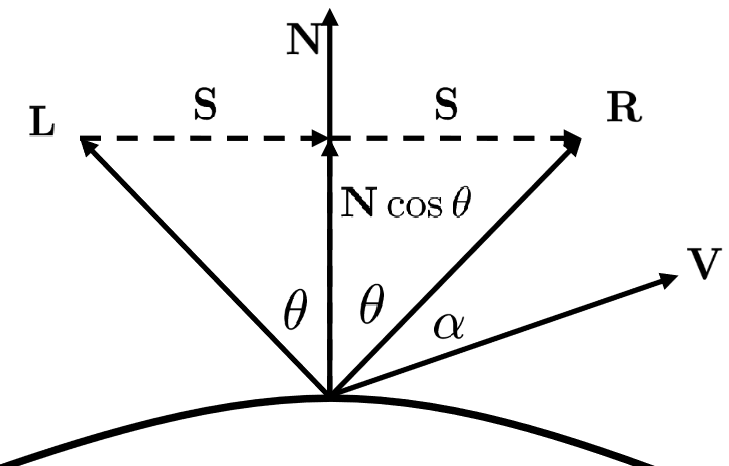
\includegraphics[width = \linewidth]{arjun/phong-illumination.png}
\end{minipage}

\subsection*{Shading}
\greenbf{Flat:} 1 color per primitive, per triangle \\
\greenbf{Gouraud:} Linearly interpolate vertex intensities
\begin{compactenum}
    \item Calculate vertex normal by averaging face normals.
    \item Evaluate illumination model for each vertex
    \item Interpolate vertex colors bilinearly on the scan line.
\end{compactenum}
\begin{center}
    \includegraphics*[width = 0.5\columnwidth]{arjun/gouraud-shading.png}
\end{center}

$I_a = I_1 - (I_1 - I_2)\frac{(y_1-y_s)}{(y_1 - y_2)}$  
$I_b = I_1 - \left(I_1 - I_3\right) \frac{\left(y_1 - y_s\right)}{\left(y_1 - y_3\right)}$ 
$I_p = I_b - \left(I_b - I_a\right) \frac{\left(x_b - x_p\right)}{\left(x_b - x_a\right)}
$

Problems: Perspective Distortion. Orientation Dependence due to interpolation. Shared Vertices.

\greenbf{Phong Shading:} Linearly interpolate normals, color per pixel
\begin{compactenum}
    \item Calculate vertex normal by averaging face normals.
    \item Interpolate the normal barycentric
    \item Evaluate illumination model per fragment in triangle
\end{compactenum}
\begin{center}
    \includegraphics*[width = 0.5\columnwidth]{arjun/phong-shading.png}
\end{center}

$ n_x = \lambda_an_a + \lambda_bn_b + \lambda_cn_c  \quad \lambda_a = \frac{\color{blue} \Delta xbc}{\Delta abc} \quad \lambda_b = \frac{\color{red} \Delta xac}{\Delta abc} \quad \lambda_c = 1 - \lambda_a - \lambda_b$ 

\subsection*{Transparency}
\greenbf{Alpha Blending:} is the linear interpolation of color front-to-back (obj. 1 is closer than obj. 2): $I = I_1 \alpha_1 + \alpha_2 I_2 (1 - \alpha_1)$\\
$\alpha = 1 $: opaque. $\alpha = 0$: transparent.\\
We render back to front, beginning with opaque object. Can cause issues with overlapping objects. Solution is depth peeling. We do multiple passes where each pass renders the next closest fragment.